
%% bare_conf.tex
%% V1.4b
%% 2015/08/26
%% by Michael Shell
%% See:
%% http://www.michaelshell.org/
%% for current contact information.
%%
%% This is a skeleton file demonstrating the use of IEEEtran.cls
%% (requires IEEEtran.cls version 1.8b or later) with an IEEE
%% conference paper.
%%
%% Support sites:
%% http://www.michaelshell.org/tex/ieeetran/
%% http://www.ctan.org/pkg/ieeetran
%% and
%% http://www.ieee.org/

%%*************************************************************************
%% Legal Notice:
%% This code is offered as-is without any warranty either expressed or
%% implied; without even the implied warranty of MERCHANTABILITY or
%% FITNESS FOR A PARTICULAR PURPOSE! 
%% User assumes all risk.
%% In no event shall the IEEE or any contributor to this code be liable for
%% any damages or losses, including, but not limited to, incidental,
%% consequential, or any other damages, resulting from the use or misuse
%% of any information contained here.
%%
%% All comments are the opinions of their respective authors and are not
%% necessarily endorsed by the IEEE.
%%
%% This work is distributed under the LaTeX Project Public License (LPPL)
%% ( http://www.latex-project.org/ ) version 1.3, and may be freely used,
%% distributed and modified. A copy of the LPPL, version 1.3, is included
%% in the base LaTeX documentation of all distributions of LaTeX released
%% 2003/12/01 or later.
%% Retain all contribution notices and credits.
%% ** Modified files should be clearly indicated as such, including  **
%% ** renaming them and changing author support contact information. **
%%*************************************************************************


% *** Authors should verify (and, if needed, correct) their LaTeX system  ***
% *** with the testflow diagnostic prior to trusting their LaTeX platform ***
% *** with production work. The IEEE's font choices and paper sizes can   ***
% *** trigger bugs that do not appear when using other class files.       ***                          ***
% The testflow support page is at:
% http://www.michaelshell.org/tex/testflow/



\documentclass[conference]{IEEEtran}
% Some Computer Society conferences also require the compsoc mode option,
% but others use the standard conference format.
%
% If IEEEtran.cls has not been installed into the LaTeX system files,
% manually specify the path to it like:
% \documentclass[conference]{../sty/IEEEtran}





% Some very useful LaTeX packages include:
% (uncomment the ones you want to load)


% *** MISC UTILITY PACKAGES ***
%
%\usepackage{ifpdf}
% Heiko Oberdiek's ifpdf.sty is very useful if you need conditional
% compilation based on whether the output is pdf or dvi.
% usage:
% \ifpdf
%   % pdf code
% \else
%   % dvi code
% \fi
% The latest version of ifpdf.sty can be obtained from:
% http://www.ctan.org/pkg/ifpdf
% Also, note that IEEEtran.cls V1.7 and later provides a builtin
% \ifCLASSINFOpdf conditional that works the same way.
% When switching from latex to pdflatex and vice-versa, the compiler may
% have to be run twice to clear warning/error messages.






% *** CITATION PACKAGES ***
%
%\usepackage{cite}
% cite.sty was written by Donald Arseneau
% V1.6 and later of IEEEtran pre-defines the format of the cite.sty package
% \cite{} output to follow that of the IEEE. Loading the cite package will
% result in citation numbers being automatically sorted and properly
% "compressed/ranged". e.g., [1], [9], [2], [7], [5], [6] without using
% cite.sty will become [1], [2], [5]--[7], [9] using cite.sty. cite.sty's
% \cite will automatically add leading space, if needed. Use cite.sty's
% noadjust option (cite.sty V3.8 and later) if you want to turn this off
% such as if a citation ever needs to be enclosed in parenthesis.
% cite.sty is already installed on most LaTeX systems. Be sure and use
% version 5.0 (2009-03-20) and later if using hyperref.sty.
% The latest version can be obtained at:
% http://www.ctan.org/pkg/cite
% The documentation is contained in the cite.sty file itself.






% *** GRAPHICS RELATED PACKAGES ***
%
\ifCLASSINFOpdf
   \usepackage[pdftex]{graphicx}
  % declare the path(s) where your graphic files are
  % \graphicspath{{../pdf/}{../jpeg/}}
  % and their extensions so you won't have to specify these with
  % every instance of \includegraphics
  % \DeclareGraphicsExtensions{.pdf,.jpeg,.png}
\else
  % or other class option (dvipsone, dvipdf, if not using dvips). graphicx
  % will default to the driver specified in the system graphics.cfg if no
  % driver is specified.
  % \usepackage[dvips]{graphicx}
  % declare the path(s) where your graphic files are
  % \graphicspath{{../eps/}}
  % and their extensions so you won't have to specify these with
  % every instance of \includegraphics
  % \DeclareGraphicsExtensions{.eps}
\fi
% graphicx was written by David Carlisle and Sebastian Rahtz. It is
% required if you want graphics, photos, etc. graphicx.sty is already
% installed on most LaTeX systems. The latest version and documentation
% can be obtained at: 
% http://www.ctan.org/pkg/graphicx
% Another good source of documentation is "Using Imported Graphics in
% LaTeX2e" by Keith Reckdahl which can be found at:
% http://www.ctan.org/pkg/epslatex
%
% latex, and pdflatex in dvi mode, support graphics in encapsulated
% postscript (.eps) format. pdflatex in pdf mode supports graphics
% in .pdf, .jpeg, .png and .mps (metapost) formats. Users should ensure
% that all non-photo figures use a vector format (.eps, .pdf, .mps) and
% not a bitmapped formats (.jpeg, .png). The IEEE frowns on bitmapped formats
% which can result in "jaggedy"/blurry rendering of lines and letters as
% well as large increases in file sizes.
%
% You can find documentation about the pdfTeX application at:
% http://www.tug.org/applications/pdftex





% *** MATH PACKAGES ***
%
%\usepackage{amsmath}
% A popular package from the American Mathematical Society that provides
% many useful and powerful commands for dealing with mathematics.
%
% Note that the amsmath package sets \interdisplaylinepenalty to 10000
% thus preventing page breaks from occurring within multiline equations. Use:
%\interdisplaylinepenalty=2500
% after loading amsmath to restore such page breaks as IEEEtran.cls normally
% does. amsmath.sty is already installed on most LaTeX systems. The latest
% version and documentation can be obtained at:
% http://www.ctan.org/pkg/amsmath





% *** SPECIALIZED LIST PACKAGES ***
%
%\usepackage{algorithmic}
% algorithmic.sty was written by Peter Williams and Rogerio Brito.
% This package provides an algorithmic environment fo describing algorithms.
% You can use the algorithmic environment in-text or within a figure
% environment to provide for a floating algorithm. Do NOT use the algorithm
% floating environment provided by algorithm.sty (by the same authors) or
% algorithm2e.sty (by Christophe Fiorio) as the IEEE does not use dedicated
% algorithm float types and packages that provide these will not provide
% correct IEEE style captions. The latest version and documentation of
% algorithmic.sty can be obtained at:
% http://www.ctan.org/pkg/algorithms
% Also of interest may be the (relatively newer and more customizable)
% algorithmicx.sty package by Szasz Janos:
% http://www.ctan.org/pkg/algorithmicx




% *** ALIGNMENT PACKAGES ***
%
%\usepackage{array}
% Frank Mittelbach's and David Carlisle's array.sty patches and improves
% the standard LaTeX2e array and tabular environments to provide better
% appearance and additional user controls. As the default LaTeX2e table
% generation code is lacking to the point of almost being broken with
% respect to the quality of the end results, all users are strongly
% advised to use an enhanced (at the very least that provided by array.sty)
% set of table tools. array.sty is already installed on most systems. The
% latest version and documentation can be obtained at:
% http://www.ctan.org/pkg/array


% IEEEtran contains the IEEEeqnarray family of commands that can be used to
% generate multiline equations as well as matrices, tables, etc., of high
% quality.




% *** SUBFIGURE PACKAGES ***
%\ifCLASSOPTIONcompsoc
%  \usepackage[caption=false,font=normalsize,labelfont=sf,textfont=sf]{subfig}
%\else
%  \usepackage[caption=false,font=footnotesize]{subfig}
%\fi
% subfig.sty, written by Steven Douglas Cochran, is the modern replacement
% for subfigure.sty, the latter of which is no longer maintained and is
% incompatible with some LaTeX packages including fixltx2e. However,
% subfig.sty requires and automatically loads Axel Sommerfeldt's caption.sty
% which will override IEEEtran.cls' handling of captions and this will result
% in non-IEEE style figure/table captions. To prevent this problem, be sure
% and invoke subfig.sty's "caption=false" package option (available since
% subfig.sty version 1.3, 2005/06/28) as this is will preserve IEEEtran.cls
% handling of captions.
% Note that the Computer Society format requires a larger sans serif font
% than the serif footnote size font used in traditional IEEE formatting
% and thus the need to invoke different subfig.sty package options depending
% on whether compsoc mode has been enabled.
%
% The latest version and documentation of subfig.sty can be obtained at:
% http://www.ctan.org/pkg/subfig




% *** FLOAT PACKAGES ***
%
%\usepackage{fixltx2e}
% fixltx2e, the successor to the earlier fix2col.sty, was written by
% Frank Mittelbach and David Carlisle. This package corrects a few problems
% in the LaTeX2e kernel, the most notable of which is that in current
% LaTeX2e releases, the ordering of single and double column floats is not
% guaranteed to be preserved. Thus, an unpatched LaTeX2e can allow a
% single column figure to be placed prior to an earlier double column
% figure.
% Be aware that LaTeX2e kernels dated 2015 and later have fixltx2e.sty's
% corrections already built into the system in which case a warning will
% be issued if an attempt is made to load fixltx2e.sty as it is no longer
% needed.
% The latest version and documentation can be found at:
% http://www.ctan.org/pkg/fixltx2e


%\usepackage{stfloats}
% stfloats.sty was written by Sigitas Tolusis. This package gives LaTeX2e
% the ability to do double column floats at the bottom of the page as well
% as the top. (e.g., "\begin{figure*}[!b]" is not normally possible in
% LaTeX2e). It also provides a command:
%\fnbelowfloat
% to enable the placement of footnotes below bottom floats (the standard
% LaTeX2e kernel puts them above bottom floats). This is an invasive package
% which rewrites many portions of the LaTeX2e float routines. It may not work
% with other packages that modify the LaTeX2e float routines. The latest
% version and documentation can be obtained at:
% http://www.ctan.org/pkg/stfloats
% Do not use the stfloats baselinefloat ability as the IEEE does not allow
% \baselineskip to stretch. Authors submitting work to the IEEE should note
% that the IEEE rarely uses double column equations and that authors should try
% to avoid such use. Do not be tempted to use the cuted.sty or midfloat.sty
% packages (also by Sigitas Tolusis) as the IEEE does not format its papers in
% such ways.
% Do not attempt to use stfloats with fixltx2e as they are incompatible.
% Instead, use Morten Hogholm'a dblfloatfix which combines the features
% of both fixltx2e and stfloats:
%
% \usepackage{dblfloatfix}
% The latest version can be found at:
% http://www.ctan.org/pkg/dblfloatfix




% *** PDF, URL AND HYPERLINK PACKAGES ***
%
%\usepackage{url}
% url.sty was written by Donald Arseneau. It provides better support for
% handling and breaking URLs. url.sty is already installed on most LaTeX
% systems. The latest version and documentation can be obtained at:
% http://www.ctan.org/pkg/url
% Basically, \url{my_url_here}.




% *** Do not adjust lengths that control margins, column widths, etc. ***
% *** Do not use packages that alter fonts (such as pslatex).         ***
% There should be no need to do such things with IEEEtran.cls V1.6 and later.
% (Unless specifically asked to do so by the journal or conference you plan
% to submit to, of course. )


% correct bad hyphenation here
%\hyphenation{op-tical net-works semi-conduc-tor}


\begin{document}
%
% paper title
% Titles are generally capitalized except for words such as a, an, and, as,
% at, but, by, for, in, nor, of, on, or, the, to and up, which are usually
% not capitalized unless they are the first or last word of the title.
% Linebreaks \\ can be used within to get better formatting as desired.
% Do not put math or special symbols in the title.
\title{Towards a Provenance-Aware Internet of Things (IoT) System}


% author names and affiliations
% use a multiple column layout for up to three different
% affiliations

%\author{\IEEEauthorblockN{Michael Shell}
%\IEEEauthorblockA{School of Electrical and\\Computer Engineering\\
%Georgia Institute of Technology\\
%Atlanta, Georgia 30332--0250\\
%Email: http://www.michaelshell.org/contact.html}
%\and
%\IEEEauthorblockN{Homer Simpson}
%\IEEEauthorblockA{Twentieth Century Fox\\
%Springfield, USA\\
%Email: homer@thesimpsons.com}
%\and
%\IEEEauthorblockN{James Kirk\\ and Montgomery Scott}
%\IEEEauthorblockA{Starfleet Academy\\
%San Francisco, California 96678--2391\\
%Telephone: (800) 555--1212\\
%Fax: (888) 555--1212}}

% conference papers do not typically use \thanks and this command
% is locked out in conference mode. If really needed, such as for
% the acknowledgment of grants, issue a \IEEEoverridecommandlockouts
% after \documentclass

% for over three affiliations, or if they all won't fit within the width
% of the page, use this alternative format:
% 
\author{\IEEEauthorblockN{
Ebelechukwu Nwafor \IEEEauthorrefmark{1},
Gedare Bloom\IEEEauthorrefmark{1}, 
Andre Campbell\IEEEauthorrefmark{1} and
David Hill\IEEEauthorrefmark{1}}
\IEEEauthorblockA{\IEEEauthorrefmark{1}Department of Electrical Engineering and Computer Science\\
Howard University,
Washington, DC 30332--0250\\ Email: ebelechukwu.nwafor@bison.howard.edu}
%\IEEEauthorblockA{\IEEEauthorrefmark{2}Twentieth Century Fox, Springfield, USA\\
%Email: homer@thesimpsons.com}
%\IEEEauthorblockA{\IEEEauthorrefmark{3}Starfleet Academy, San Francisco, California 96678-2391\\
%Telephone: (800) 555--1212, Fax: (888) 555--1212}
%\IEEEauthorblockA{\IEEEauthorrefmark{4}Tyrell Inc., 123 Replicant Street, Los Angeles, California 90210--4321}
}




%\author{\IEEEauthorblockN{Ebelechukwu Nwafor\IEEEauthorrefmark{1},
%Gedare Bloom\IEEEauthorrefmark{2}, Andre Campbell\IEEEauthorrefmark{3} and
%David Hill\IEEEauthorrefmark{4}}
%\IEEEauthorblockA{Department of Electrical Engineering and Computer Science\\
%\\ 2366 Sixth Street, NW, Washington, DC 20059\\
%Email: \IEEEauthorrefmark{1}ebelechukwu.nwafor@bison.howard.edu,
%\IEEEauthorrefmark{2}gedare@scs.howard.edu,
%\IEEEauthorrefmark{3}author.three@add.on.net,
%\IEEEauthorrefmark{4}author.four@add.on.net}}


% use for special paper notices
%\IEEEspecialpapernotice{(Invited Paper)}




% make the title area
\maketitle

% As a general rule, do not put math, special symbols or citations
% in the abstract
\begin{abstract}
The Internet of Things (IoT) offers immense benefits by enabling devices
to leverage networked resources theryby making intelligent decisions. The
numerous heterogeneous connected devices that exist throughout the IoT
system creates new security and privacy concerns. Some of these concerns
can be overcome through trust, transparency, and integrity, which can be
achieved with data provenance. Data provenance, also known as data lineage,
provides a history of transformations that occurs on a data object
from the time it was created to its current state. Data provenance has been
explored in the areas of scientific computing, business, forensic analysis, and
intrusion detection. Data provenance can help in detecting and mitigating
malicious cyber attacks. In this paper, we explore the integration of provenance within the IoT.
We propose a provenance collection framework for IoT applications. We evaluate the effectiveness
of our framework by looking at an application of provenance data by developing a prototype system for proof of concept.
\end{abstract}

% no keywords




% For peer review papers, you can put extra information on the cover
% page as needed:
% \ifCLASSOPTIONpeerreview
% \begin{center} \bfseries EDICS Category: 3-BBND \end{center}
% \fi
%
% For peerreview papers, this IEEEtran command inserts a page break and
% creates the second title. It will be ignored for other modes.
\IEEEpeerreviewmaketitle



\section{Introduction}
% no \IEEEPARstart
The Internet of Things (IoT) has generated a lot of buzz among commercial and industrial information technology experts all over the world.  Heterogeneous devices like we have never seen before are communicating with each other over a shared network (e.g internet). For example, It is possible to automatically control the temperature of a house remotely though a cell phone. 

IoT offers a lot of benefits in the areas of home and industrial automation which makes operations which might require a lot of interaction seamless.


however, with this unprecedented communication, here has been an exponential increase in the number of devices connected to the internet. It is estimated that over 50 million devices will be connected to the internet by the year 2020. With the vast amounts of connected heterogeneous devices, security and privacy risks is increased. IoT devices are not strongly incorporated with security in mind. This raises the complexity of including security after the device has been deployed. For instance some devices come with default passwords which might never be changed during its lifecycle. The vast amount of data generated from IoT
devices requires stronger levels of trust which can be achieved through data
provenance.


Data provenance is a comprehensive history of activities that occurred on an entity from its origin to its current state. Provenance ensures integrity of data . Provenance has been applied in various area such as scientific workflow for experiment reproducibility, and information security as a form of access control and also for intrusion detection in mitigating malicious adversaries.  Provenance ensure trust and integrity of data. IoT devices (things) produces sensor-actuator data. A workflow representation of of how sensor data is generated can be generated to depict dependency between sensor-actuator readings and devices/sensor information contained in the device. \par This information generated can be prove to be beneficial as a means for mitigating malicious intrusion or for scientific reproducability as provenance. In this paper, we propose a provenance aware framework for IoT devices, in which provenance data is collected and modeled to represent dependencies between sensor-actuator readings and the various entities contained in the IoT architecture. Most of the interconnected heterogeneous devices (things) are embedded systems which require lightweight and efficient solutions as compared to general purpose
systems. This requirement is attributed to the constrained memory and computing power of such
devices. 

The remaining section of the paper is organized as follows: section 2 discusses background information on IoT definition, architecture ,application domain and data provenance. Section 3 discusses the need for a incoporating provenance to IoT using a use case scenario of an automated smart home. Section 3 talks about related work in provenance collection systems. Section 4 discusses implementation details for provenance collection framework. Section 5 talks about results and experiment analysis. Finally, in section 6 we conclude with future work.


\section{Background} 
This section describes key concepts of data provenance, IoT characteristics, and provenance models. It also provides motivating example for the need for provenance collection via a use case.

\subsection{Internet of Things}
There is no standard definition for IoT, however, researchers have tried to define the concept
of connected \"things\". The concept of IoT was proposed by Mark Weiser in the early 1990s
 which represents a way in which the physical objects, \" things\", can be connected to the
digital world. Gubbi et al defines the IoT as an interconnection of sensing and actuating
devices that allows data sharing across platforms through a centralized framework. We
define (IoT) as follows:  

The Internet of Things (IoT) is a network of heterogeneous devices with sensing and actuating capabilities communicating over the internet.

%\newtheorem{definition}{Definition}
%
%\begin{definition}
%
%The Internet of Things (IoT) is a network of heterogeneous devices with
%sensing and actuating capabilities communicating over the internet.
%
%\end{definition}


\par IoT has applications in home automation, smart health, automotive communication, machine to machine comminication, industrial automation. The notion of IoT has been attributed to smart devices. The interconnectivity between various heterogeneous devices allows for devices to share information in a unique manner.
Analytics is a driving force for IoT. With analytics, devices can learn from user data
to make smarter decisions. This notion of smart devices is seen in various commercial
applications such as smartwatches, thermostats that automatically learns a user patterns. The ubiquitous nature of these devices make them ideal choices to be included in consumer products.  IoT architecture represents a functional hierarchy of how information is disseminated across
multiple hierarchies contained in an IoT framework; from devices which contain sensing and
actuating capabilities to massive data centers (cloud storage). Knowing how information
is transmitted across layers allows a better understanding on how to model the flow of
information across actors contained in an IoT hierarchy.
Figure 1 displays the IoT architecture and the interactions between the respective
layers. IoT architecture consists of four distinct layers: The sensor and actuator layer, device layer, gateway layer and the cloud layer. The base of the architectural stack consist of sensors and actuators which gathers provenance information and interacts with the device layer. The device layer consists of
devices (e.g mobile phones, laptops, smart devices) which are responsible for aggregating
data collected from sensors and actuators. These devices in turn forwards the aggregated
data to the gateway layer. The gateway layer routes and forwards data collected from the
device later. It could also serve as a medium of temporary storage and data processing.
The cloud layer is involved with the storage and processing of data collected from the
gateway layer. Note that the resource constraints decreases up the architectural stack with
the cloud layer having the most resources (memory, power computation) and the sensor-
actuator layer having the least. 




\begin{figure}[h]
\begin{center}

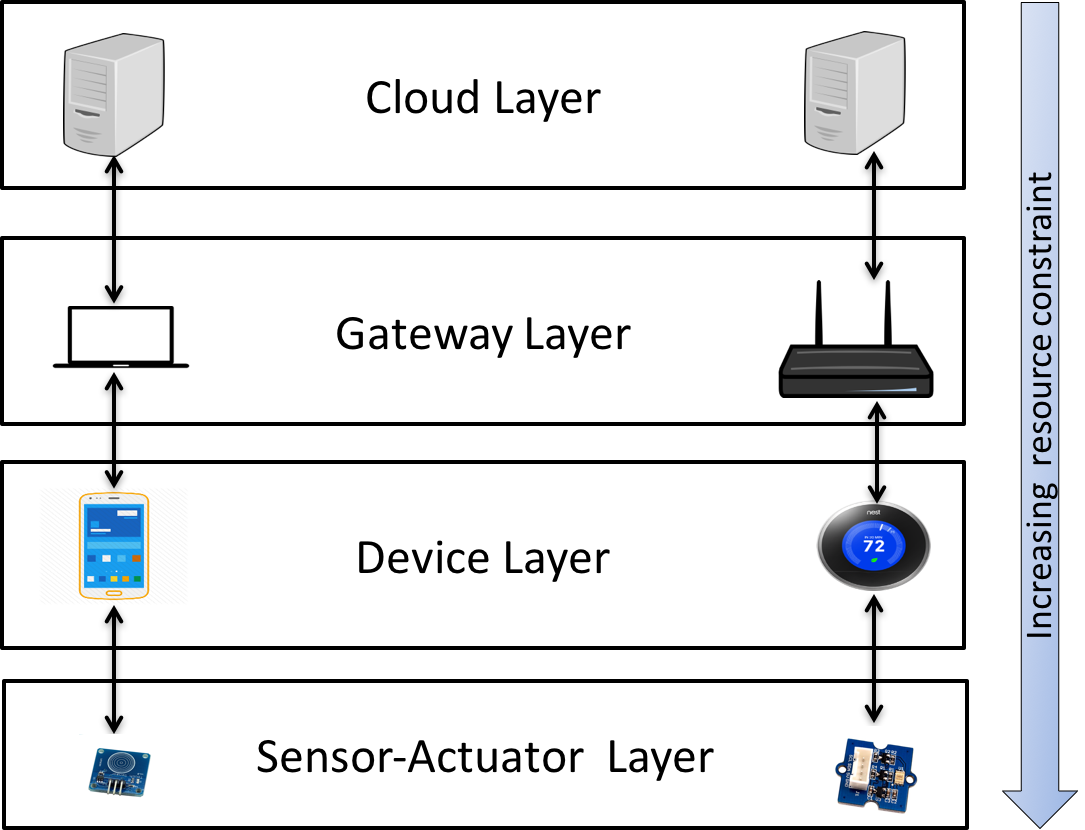
\includegraphics[height=2.0in]{iot_architecture.png}
\end{center}
\caption{IoT Architecture Diagram. The arrows illustrates the interaction between data at various layers on the architecture.}
\label{iot_architecture}

\end{figure}

With the recent data explosion [22] due to the large influx  in amounts of interconnected devices, information is disseminated at a fast rate and with this increase involves security and privacy concerns. Creating a provenance-aware system is beneficial to IoT because it
ensures the trust and integrity of interconnected devices. Enabling provenance collection in IoT devices allows these devices to capture valuable information which enables backtracking in an event of a malicious attack. 


\subsection{Provenance-Aware IoT Device Use Case}

\begin{figure}[h]
\begin{center}
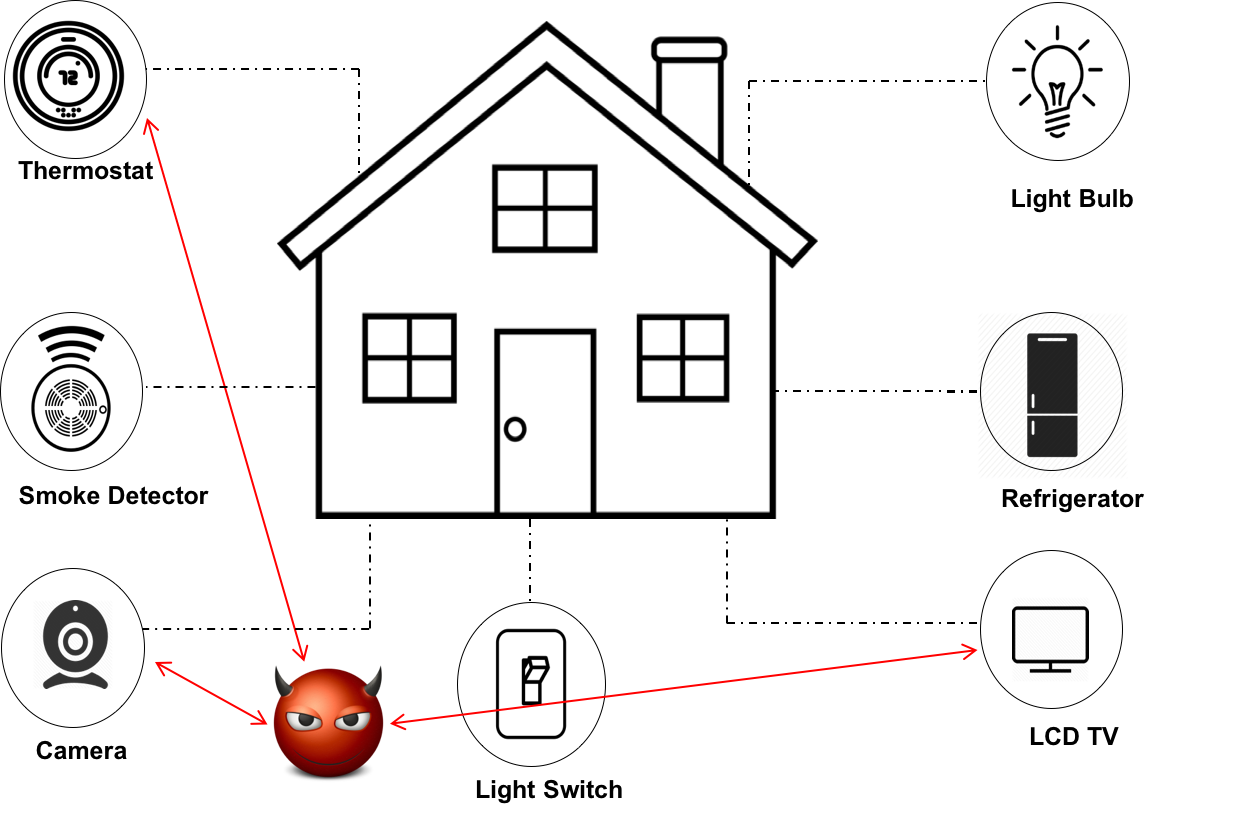
\includegraphics[height=2.5in]{smart_home.png}
\end{center}
\caption{Smart home use case Diagram}
\label{smart_home}
\end{figure}



Consider a smart home as illustrated in Figure \ref{smart_home} that contains interconnected devices such as a thermostat which automatically detects and regulates the temperature of a room based on prior information of a user's temperature preferences, a smart lock system that can be controlled remotely and informs a user via short messaging when the door has been opened or is closed, a home security camera monitoring system, a smart fridge which sends a reminder when food products are low. In an event that a malicious intruder attempts  to gain access to the smart lock system and security camera remotely, provenance information can be used to track the series  of events to determine where and how a malicious attack originated. Provenance can also be used as a safeguard to alert of a possible remote or insider compromise thereby protecting against future or ongoing malicious attacks. 



\subsection{Data Provenance}

The Oxford English dictionary defines provenance as the place of origin or earliest
known history of something". An example of provenance can be seen with a college transcript. A transcript is the provenance of a college degree because it outlines all of the
courses satisfied in order to attain the degree. In the field of computing, data provenance, also known as data lineage, can be defined as the history of all activities performed on entities from its creation to its current state.
Cheney et al.  describes provenance as the origin and history of data from its lifecycle. Buneman et al describes provenance from a database perspective as the origin of data and the steps in which it is derived in the database system. We formally define provenance as follows:  Data provenance of an entity is a comprehensive history of activities that occur on that entity from its creation to its present state.

%\begin{definition}
%Data provenance of an entity is a comprehensive history of activities that occur on that entity from its creation to its present state.
%\end{definition}

\par Provenance ensures trust and integrity of data \cite{Bertino2015}. It outlines dependency between all objects involved in the system and allows for the verification of the source of data. dependency is used to determine the relationship between multiple objects. The relationship in which provenance denotes can in turn be used in digital forensics \cite{zawoadfecloud} to investigate the cause of a malicious attack and also in intrusion detection systems to further enhance the security of computing devices. Provenance has been utilized in application domains such as computer security for access control and intrusion detection, in scientific experiments for reproducability  and in version control systems to mention but a few. 
 
 \subsubsection{Provenance Characteristics}

Since provenance denotes the who, where and why of data transformation, it is imperative that data disseminated in an IoT architecture satisfies the required conditions. The characteristics of data provenance are outlined in detail below.


\begin{itemize}

\item Who: This characteristic provides information on activities made to an entity. Knowing the ``who" characteristic is essential because it maps the identity of modification to a particular data object. An example of ``who" in an IoT use case is a sensor device identifier.

\item Where: This characteristic denotes location information in which data transformation was made. This provenance characteristic could be optional since not every data modification contains location details.

\item When: This characteristic denotes the time information at which data transformation occurred. This is an essential provenance characteristic. Being able to tell the time of a data transformation allows for tracing data irregularities.

\item What: This characteristic denotes the transformation is applied on a data object. A use case for IoT can be seen in the various operations (create, read, update, and delete) that could be performed on a file object.

\end{itemize}

\subsubsection{Differentiating Provenance, Log data, and Metadata }

Provenance has often been seen used interchangably to define log data, and metadata. While some overlap exists between the three, some differences exists. Log data contains information about the activities of an operating system or processes. Log data can be used as provenance because It contains data trace specific to an application domain. Log files might contain unrelated information such as error messages, warnings which might not be considered as provenance data. Provenance allows for specified collection of information that relates to the change of the internal state of an object. In summary, log data could provide insight to what provenance data to collect. 


\subsection{Model for representing provenance for IoT}

In order to represent the right kind of provenance information in an IoT architecture, we need to satisfy the who, where, how, and what of data transformations. The provenance of sensor and actuator data in an IoT device showing the depency between all entities responsible for generating the sensor reading. 



Provenance data can be represented using a provenance model in a modeling language such as, PROV\-DM which is represented in serialized in three format:  XML, JSON and RDF. This model displays data dependency between data objects. We propose a model that contains information such as sensor readings, device name, and device information. There are two widely accepted modeling languages for representing provenance, PROV-DM \cite{prov_dm} and  Open Provenance Model \cite{moreau_open_2011} that have been applied in various literature and are considered standard for representing provenance. Details on the provenance models are outlined below.

\subsubsection{Provenance Data Model (Prov-DM)}

PROV-DM is a model that conforms to PROV ontology. It is a W3C standard that is used to depict dependencies between entities, activities and agents (digital or physical). It creates a common model that allows for interchange of provenance information between heterogeneous devices. It contains two major components: types and relations. 


\begin{itemize}

\item Entity: An entity is a physical or digital object. An example of an entity is a file system, a process, or an motor vehicle. An entity may be physical or abstract.

\item Activity: An activity represents some form of action that occurs over a time frame. Actions are acted upon by an agent. An example of an activity is a process opening a file directory, Accessing a remote server.

\item Agent: An agent is a thing that takes ownership of an entity, or performs an activity. An example of an agent is a person, a software product, or a process.
\end{itemize}

The figure below illustrates the various types contained in PROV-DM and their representation. Entities, activities and agents are represented by oval, rectangle and hexagonal shapes respectively.

\begin{figure}[h]
\begin{center}

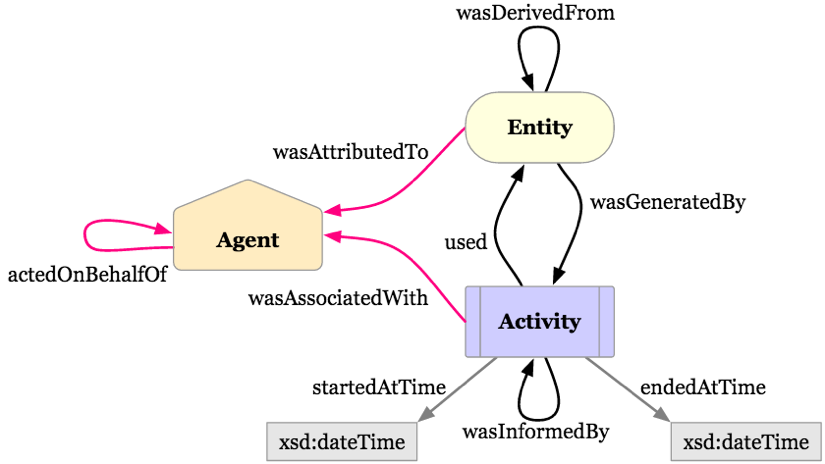
\includegraphics[width=3.0in]{prov_dm.PNG}
\end{center}
\caption{Prov-DM respresentation showing various types contained in the model (Entity, Activity, and Agent) }
\end{figure}

PROV-DM does not keep track of future events. PROV-DM relations are outlined below:


\begin{itemize}
\item wasGeneratedBy: This relation signifies the creation of an entity by an activity. 

\item used: This relation denotes that the functionality of an entity has been adopted by an activity.

\item wasInformedBy: This relation denotes a causality that follows the exchange of two activities.

\item wasDerivedFrom: This relation represents a copy of information from an entity. 

\item wasAttributedTo: This denotes relational dependency to an agent. It is used to denote relationship between entity and agent when the activity that created the agent is unknown.

\item wasAssociatedWith: This relation denotes a direct association to an agent for an activity that occurs. This indicates that an agent plays a role in the creation or modification of the activity.

\item actedOnBehalfOf: This relation denotes assigning authority to perform a particular responsibility to an agent. This could be by itself or to another agent.



\end{itemize}

\subsection {Prov-Sensor Model Alignment}

\par Using the PROV-O, In an IoT  device connected to multiple sensors while generating sensor readings in realtime, the device and the sensors are considered agents (prov:agents), the operation performed on the data (read, create, update) is considered as an activity (prov:activity). The data being generated is known as an entity (prov:entity). Sensor readings generated from the IoT device are represented as a tuple $<t, d, s_1, r_1>$ where $t$ represents a timestamp, $d$ represents data which is being collected, $s_1$ represents sensor information and $r_1$ represents device information. $d$ can alsso be a list of data points e.g Consider sensor $s_1$,  a sensor that generates sensor and humidity readings mounted device $r_1$, raspberry pi, $d$ can be defined as $d= [temperature, humidity]$ therefore the tuple representation for the IoT device $r_1$ with sensor $s_1$ is $<t, [temperature, humidity], s_1, r_1>$. Figure \ref{prov_sensor} displays a pictorial representation of the provenance sensor alignment for a device connected to three sensors $s_1, s_2, and s_3$ with data \{$d_1,...,d_4, e1, e2, f_1,...,f_4$\}.


\begin{figure}[h]
\begin{center}

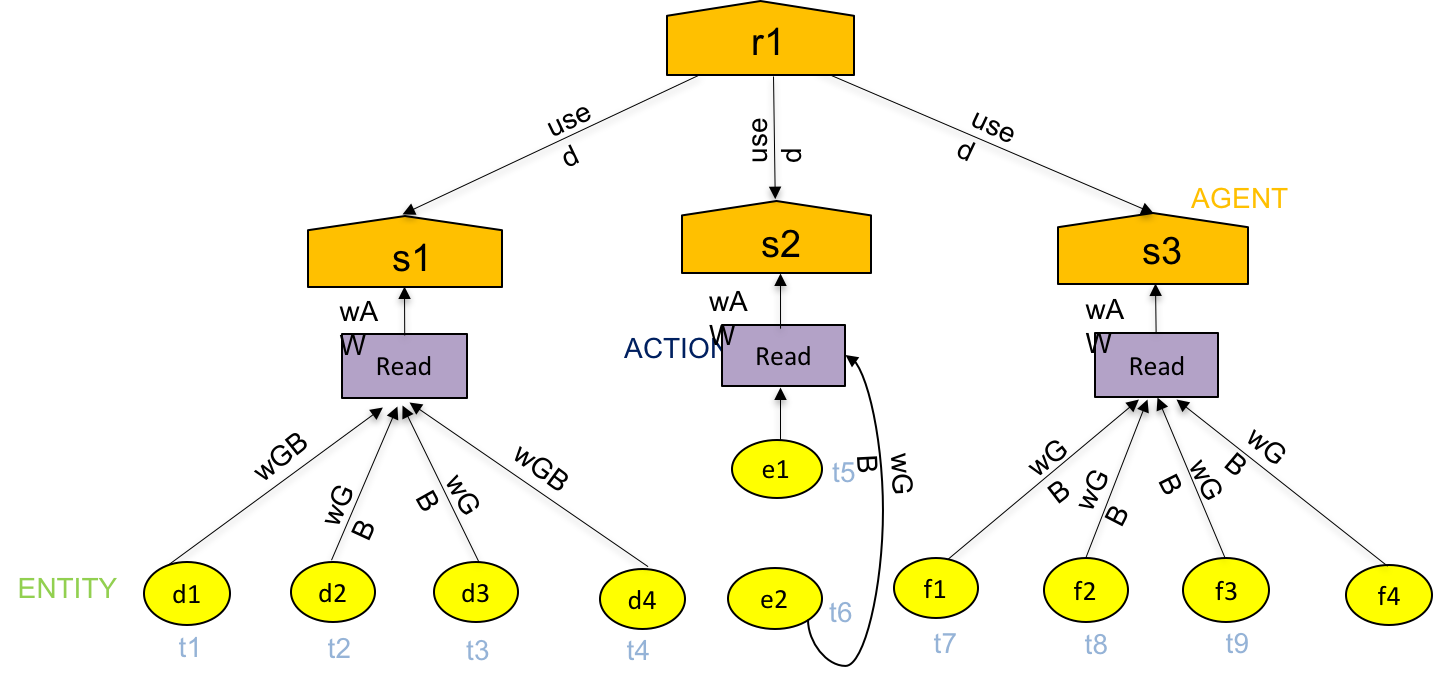
\includegraphics[width=3.5in]{prov_sensor.PNG}
\end{center}
\caption{Prov-Sensor Model Alignment }
\label{prov_sensor}
\end{figure}

% An example of a floating figure using the graphicx package.
% Note that \label must occur AFTER (or within) \caption.
% For figures, \caption should occur after the \includegraphics.
% Note that IEEEtran v1.7 and later has special internal code that
% is designed to preserve the operation of \label within \caption
% even when the captionsoff option is in effect. However, because
% of issues like this, it may be the safest practice to put all your
% \label just after \caption rather than within \caption{}.
%
% Reminder: the "draftcls" or "draftclsnofoot", not "draft", class
% option should be used if it is desired that the figures are to be
% displayed while in draft mode.
%
%\begin{figure}[!t]
%\centering
%\includegraphics[width=2.5in]{myfigure}
% where an .eps filename suffix will be assumed under latex, 
% and a .pdf suffix will be assumed for pdflatex; or what has been declared
% via \DeclareGraphicsExtensions.
%\caption{Simulation results for the network.}
%\label{fig_sim}
%\end{figure}

% Note that the IEEE typically puts floats only at the top, even when this
% results in a large percentage of a column being occupied by floats.


% An example of a double column floating figure using two subfigures.
% (The subfig.sty package must be loaded for this to work.)
% The subfigure \label commands are set within each subfloat command,
% and the \label for the overall figure must come after \caption.
% \hfil is used as a separator to get equal spacing.
% Watch out that the combined width of all the subfigures on a 
% line do not exceed the text width or a line break will occur.
%
%\begin{figure*}[!t]
%\centering
%\subfloat[Case I]{\includegraphics[width=2.5in]{box}%
%\label{fig_first_case}}
%\hfil
%\subfloat[Case II]{\includegraphics[width=2.5in]{box}%
%\label{fig_second_case}}
%\caption{Simulation results for the network.}
%\label{fig_sim}
%\end{figure*}
%
% Note that often IEEE papers with subfigures do not employ subfigure
% captions (using the optional argument to \subfloat[]), but instead will
% reference/describe all of them (a), (b), etc., within the main caption.
% Be aware that for subfig.sty to generate the (a), (b), etc., subfigure
% labels, the optional argument to \subfloat must be present. If a
% subcaption is not desired, just leave its contents blank,
% e.g., \subfloat[].


% An example of a floating table. Note that, for IEEE style tables, the
% \caption command should come BEFORE the table and, given that table
% captions serve much like titles, are usually capitalized except for words
% such as a, an, and, as, at, but, by, for, in, nor, of, on, or, the, to
% and up, which are usually not capitalized unless they are the first or
% last word of the caption. Table text will default to \footnotesize as
% the IEEE normally uses this smaller font for tables.
% The \label must come after \caption as always.
%
%\begin{table}[!t]
%% increase table row spacing, adjust to taste
%\renewcommand{\arraystretch}{1.3}
% if using array.sty, it might be a good idea to tweak the value of
% \extrarowheight as needed to properly center the text within the cells
%\caption{An Example of a Table}
%\label{table_example}
%\centering
%% Some packages, such as MDW tools, offer better commands for making tables
%% than the plain LaTeX2e tabular which is used here.
%\begin{tabular}{|c||c|}
%\hline
%One & Two\\
%\hline
%Three & Four\\
%\hline
%\end{tabular}
%\end{table}


% Note that the IEEE does not put floats in the very first column
% - or typically anywhere on the first page for that matter. Also,
% in-text middle ("here") positioning is typically not used, but it
% is allowed and encouraged for Computer Society conferences (but
% not Computer Society journals). Most IEEE journals/conferences use
% top floats exclusively. 
% Note that, LaTeX2e, unlike IEEE journals/conferences, places
% footnotes above bottom floats. This can be corrected via the
% \fnbelowfloat command of the stfloats package.

\section{Related Works}

There has been a considerable amount of work done on data provenance collection \cite{_general-purpose_2012, bates_trustworthy_2015, gessiou_towards_2012, muniswamy_reddy_provenance_2010}. Some of the work done has been focused on databases, sensor networks, scientific workflow systems and file system provenance but so far little attention has been given to provenance in IoT. Some of the prior work done on data provenance collection are outlined below:

\subsection{Provenance Aware Storage System (PASS)}
Muniswamy Reddy
et al \cite{muniswamy_reddy} developed a provenance collection system that tracks  system\-level provenance of the Linux file system. Provenance information
is stored in the same location as the file system for easy accessibility, backup,
restoration, and data management. Provenance information is collected and stored in
the kernel space. PASS is composed of 3 major components: provenance collector, provenance storage,and provenance query. The collector keeps track of system level provenance. It intercepts system calls which are translated into provenance data and initially stored in memory as inode cache. Provenance data is then transferred to a file system in an kernel database, BerkleyDB. This database maps key value pairs for provenance data for fast index look up. PASS collects and stores provenance information containing a reference to the executable that created the provenance data, input files, a description of hardware in which provenance data is produced, OS information, process environment, process parameters, and other data such as a random number generator seed. PASS detects and eliminates cycles that might occur in provenance dependencies as a result of version avoidance. Cycles violate the dependency relationships between entities. For example, a child node could depend on a parent node and also be an ancestor of a parent node. PASS eliminates cycles by merging processes that might have led to the cycles. It also provides functionality for querying provenance data in the database. The query tool is built on top of BerkleyDB. For querying provenance, users can process queries using the provenance explorer. Query is done using commands such as MAKEFILE  GENERATION which creates the sequence of events that led to the final state of a file or process. DUMP ALL, gets the provenance of the requested file.


 
\par Our approach looks at data provenance with data pruning as a key requirement since we are dealing with devices with limited memory and storage capabilities. We employ a policy based approach which allows provenance pruning by storing what provenance data is considered important to a specific organization. Also,unlike PASS, our system collects not just system level provenance but also application level provenance.

\subsection{HIFI}

Bates et al. \cite{hi_fi}  developed system level provenance collection framework for the Linux kernel using Linux Provenance Modules(LPM), this framework tracks system level provenance such as interprocess communication, networking, and kernel activities. This is achieved by mediating access to kernel objects using Linux Security Model(LSM) which is a framework that was designed for providing custom access control into the Linux kernel. It consists of a set of hooks which executed before access decision is made. LSM was designed to avoid problem created by direct system call interception. The provenance information collected from the kernel space is securely transmitted to the provenance recorder in the user space. 
\par HiFi contains three components: provenance collector, provenance log and provenance handler. The collector and log are contained in the kernel space while the handler is contained in the user space. The log is a storage medium which transmits the provenance data to the user space. The collector uses LSM which resides in the kernel space. The collector records provenance data and writes it to the provenance log. The handler reads the provenance record from the log. This approach to collecting provenance data differs from our work since we focus on embedded systems and are concerned with input and output (I/O) data, which involves sensor and actuator readings. Additionally,  HiFi deals with collecting system level events which might incur additional overhead when compared to collecting application level provenance. HiFi is engineered to work solely on the Linux operating system. Embedded systems that do not run on Linux OS will not be able to incorporate HiFi. 

\subsection{RecProv}

RecProv \cite{rec_prov} is a provenance system which records user-level provenance, avoiding the overhead incurred by kernel level provenance recording. It does not require changes to the kernel like most provenance monitoring systems. It uses Mozilla rr to perform deterministic record and replay by monitoring system calls  and non deterministic input. Mozilla rr is a debugging tool for Linux browser. It is developed for the deterministic recording and replaying of the Firefox browser in Linux. Recprov uses PTRACE\_PEEKDATA from ptrace to access the dereferenced address of the traced process from the registers. Mozilla rr relies on ptrace, which intercepts system calls to monitor the CPU state during and after a system call. It ptrace to access the dereferenced address of the traced process from the registers. System calls are monitored for file versioning. The provenance information generated is converted into PROV-JSON, and stored in Neo4j, a graph database for visualization and storage of provenance graphs. 

\subsection{Trustworthy Whole System Provenance for Linux Kernel}

Bates et al \cite{bates_towards_2013} provide a security model for provenance collection in the linux kernel. This is achieved by creating a Linux Provenance Model (LPM). LPM serves as a security layer which provides a security abstraction for provenance data. It is involved in the attestation disclosure of the application layer and authentication channel for the network layer. The goal of LPM is to provide an end to end provenance capture system. LPM ensures the following security guarantees: For LPM,the system must be able to detect and avoid malicious forgery of provenance data. The system must be trusted and easily verifiable. \par When an application invokes a system call, the LPM tracks system level provenance which is transmitted to the provenance module via a buffer. The provenance module registers contain hooks which records system call events. These events are sent to a provenance recorder in the user space. The provenance recorder ensures that the provenance data is stored in the appropriate backend of choice. Provenance recorders offer storage support for Gzip, PostGreSQL, Neo4j and SNAP.

\subsection{StoryBook}
Spillance et al \cite{story} developed a user space provenance collection system, Storybook, which allows for the collection of provenance data from the user space thereby reducing performance overhead. This system takes a modular approach that allows the use of application specific extensions allowing additions such as database provenance, system provenance, and web and email servers. It achieves provenance capture intercepting system level events on FUSE, a file system and MySQL , a relational database. StoryBook allows developers to implement provenance inspectors these are custom provenance models which captures the provenance of specific applications which are often modified by different application(e.g web servers, databases). When an operation is performed on a data object, the appropriate provenance model is triggered and provenance data for that data object is captured. StoryBook stores provenance information such as open, close, read or write, application specific provenance, and causality relationship between entities contained in the provenance system. Provenance data is stored in key value pairs using Stasis and Berkely DB as the storage backend. It also allows the use of interoperable data specifications such as RDF to transfer data between various applications. Storybook allows for provenance query by looking up an inode in the ino hashtable. Collecting application level and kernel level events is similar to our approach of provenance collection, however, our approach integrates the use of a policy to eliminate noisy provenance data thereby allowing only relevant provenance to be stored.

\subsection{Backtracking Intrusions}
Samuel et al \cite{King:2003:BI:945445.945467} developed a system, Backtracker, which generates an information flow of OS objects (e.g file, process) and events (e.g system call) in a computer system for the purpose of intrusion detection. From a detection point, information can be traced to pinpoint where a malicious attack occurred. The information flow represents a dependency graph which illustrates the relationship between system events. Detection point is a point in which an intrusion was discovered. Time is included in the dependency between objects to reduce false dependencies. Time is denoted by an increasing counter. The time is recorded as the difference of when a system call is invoked till when it ends. Backtracker is composed of two major components: EventLogger and GraphGen. An EventLogger is responsible for generating system level event log for applications running on the system. EventLogger is implemented in two ways: using a virtual machine and also as a stand alone system. In a virtual machine, the application and OS is run within a virtual machine. The OS running inside of the virtual machine is known as the guest OS while the OS on the bare-metal machine is known as the host OS, hypervisor or virtual machine monitor. The virtual machine alerts the EventLogger in the event that an application makes a system call and or exits. EventLogger gets event information, object identities, dependency relationship between events from the virtual machine's monitor and also the virtual machine's physical memory. EventLogger stores the collected information as a compressed file. EventLogger can also be implemented as a stand alone system which is incorporated in an operating system. Virtual machine is preferred to a standalone system because of the use of virtual machine allows ReVirt to be leveraged. ReVirt enables the replay of instruction by instruction execution of virtual machines. This allows for whole information capture of workloads. After the information has been captured by the EventLogger, GraphGen is used to produce visualizations that outlines the dependencies between events and objects contained in the system. GraphGen also allows for pruning of data using regular expressions which are used to filter the dependency graph and prioritize important portions of the dependency graph.

\subsection{Provenance Recording for Services}
Grouth et al \cite{groth} developed a provenance collection system, PReServ which allows software developers to integrate provenance recording into their applications. They introduce P-assertion recording protocol as a way of monitoring process  documentation for Service Oriented Architecture (SOA) in the standard for grid systems. PReServ is the implementation of P-assertion recording protocol (PreP). PreP specifies how provenance can be recorded. PReServ contains a provenance store web service for recording and querying of P-assertions. P-assertions are provenance data generated by actors about the application execution. It contains information about the messages sent and received as well as state of the message. PReServ is composed of three layers, the message translator which is involved with converting all messages received via HTTP requests to XML format for the provenance store layer. The message translator also determines which plug-in handle to route incoming request to, the  Plug-Ins layer. It implements functionality that the Provenance Store component provides. This component allows third party developers to add new functionality to store provenance data without going through details of the code implementation. The backend component stores the P-assertions. Various backend implementations could be attached to the system by the plug-in component.

\par PReServ was developed to address the needs of specific application domain (Scientific experiments). It deals with recording process documentation of Service Oriented Architecture (SOA) and collects P-assertions which are assertions made about the execution (i.e messages sent and received, state information) of actions by actors. The provenance collected by PReServ does not demonstrate causality and dependency between objects. In other words, the provenance data collected are not represented using a provenance model (e.g PROV-DM) that depicts causal relationship between provenance data. 

\subsection{Provenance-Based Trustworthiness Assessment in Sensor Networks}
Lim et al. \cite{lim} developed a
model for calculating the trust of nodes contained in a sensor network by using data
provenance and data similarity as deciding factors to calculate trust. The value of
provenance signifies that the more similar a data value is, the higher the trust score.
Also, the more the provenance of similar values differ, the higher their trust score. The trust score of a system is affected by the trust score of the sensor that forwards data to the system. Provenance is determined by the path in which data travels through the sensor network. This work differs from our approach since the authors focus on creating a trust score
of nodes connected in a sensor network using data provenance and do not emphasize
how the provenance data is collected. We are focused on creating a
provenance aware system for sensor-actuator I/O operations which may be used to ensure trust of
connected devices. 

\section*{Provenance-Aware System Implementation}

In this section, we outline components the provenance collection system and describe how provenance trace is collected across the IoT framework. Figure \ref{architecture} displays the system architecture of our approach. Sensor and actuator readings in the form of input and output (I/O) events are recorded by the tracer component. This component intercepts system level I/O events and produces trace information represented in Common Trace Format (CTF). CTF encodes binary trace output information containing multiple streams of binary events such as I/O activity. Trace information is converted to provenance data in the PROV-DM IoT model and serialized to PROV-JSON. CTF conversion to PROV-DM will be achieved using babeltrace. This conversion can happen at any layer of the IoT stack. Babeltrace is a plugin framework which allows the conversion of CTF traces into other formats. Trace or provenance data is securely transmitted to a gateway and later transmitted and stored in a cloud backend. Our backend of choice is Neo4j, a graph database for efficient storage, query and visualization of provenance data.


\begin{figure}[b]
\begin{center}

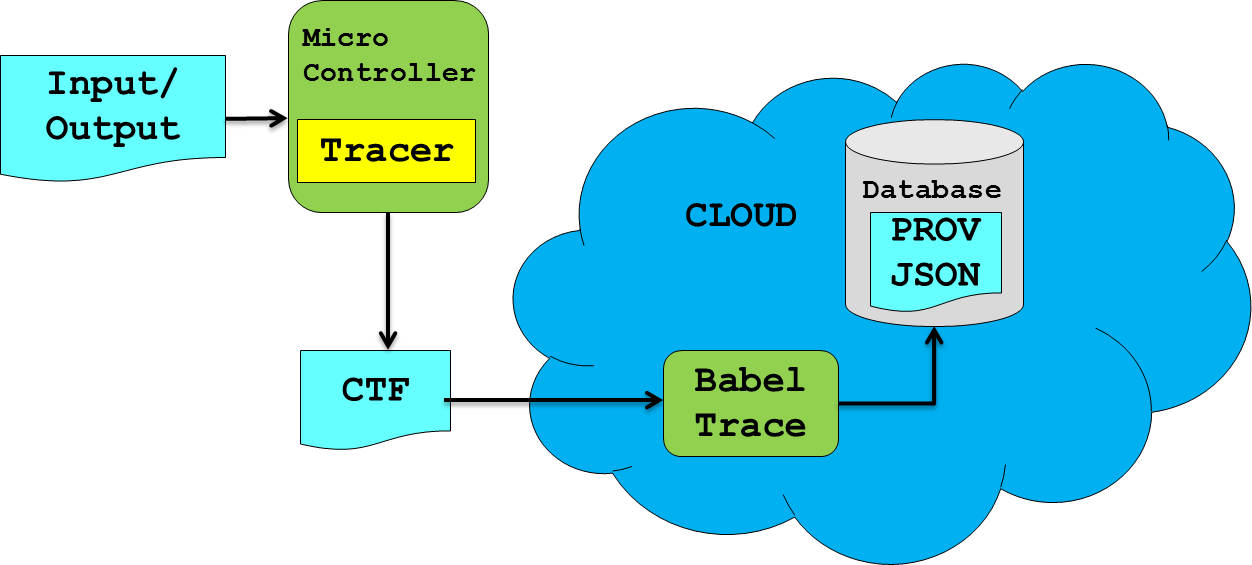
\includegraphics[width =3.0in]{system_architecture.PNG}    
\end{center}
\caption{System Architecture for Provenance Collection.}
\label{architecture}
\end{figure}

Our goal is to create a provenance-aware system which records I/O operations on data for devices connected in an IoT system. For our implementation, several tools and hardware components are utilized in the development of our prototype, outlined below:

\begin{itemize}
\item Raspberry Pi the microcontroller used to evaluate our approach. We choose Raspberry Pi because it is a representation of what can be found on an IoT gateway device and it has the capability to include custom hardware in programmable logic. Also, Raspberry Pi is a low cost, simple IoT demonstrator that was chosen for its high performance, on­board emulation, and IoT gateway projects can be programmed without additional need for hardware tools.

%\item Real Time Executive for Multiprocessor Systems (RTEMS) is an open source real­time operating system (RTOS) for embedded systems. This operating system is a typical RTOS that may be deployed in IoT devices.

\item Neo4j, a graph database which allows optimized querying of graph data. Since provenance represents causal dependencies, it is ideal to use a graph database to store the relationships between objects

%\item lttng, a software tool for collecting system level trace on Linux system. 

\item Babeltrace:  This is a trace converter tool. It contains plugins used to convert traces from one format into another. 

\item barectf: This is an application that collects bare metal application trace in CTF.

\item yaml generator: yaml generator creates yaml files. A yaml configuration file contains information on what barectf application needs in order to generate CTF trace output. This consist of configuration settings such as an application trace stream, packet type, payload type and size. 

%\item rasberrypi

\end{itemize}

\subsection{Prov-Aware IoT Information Flow }

Place holder...

\begin{figure}[h]
\begin{center}

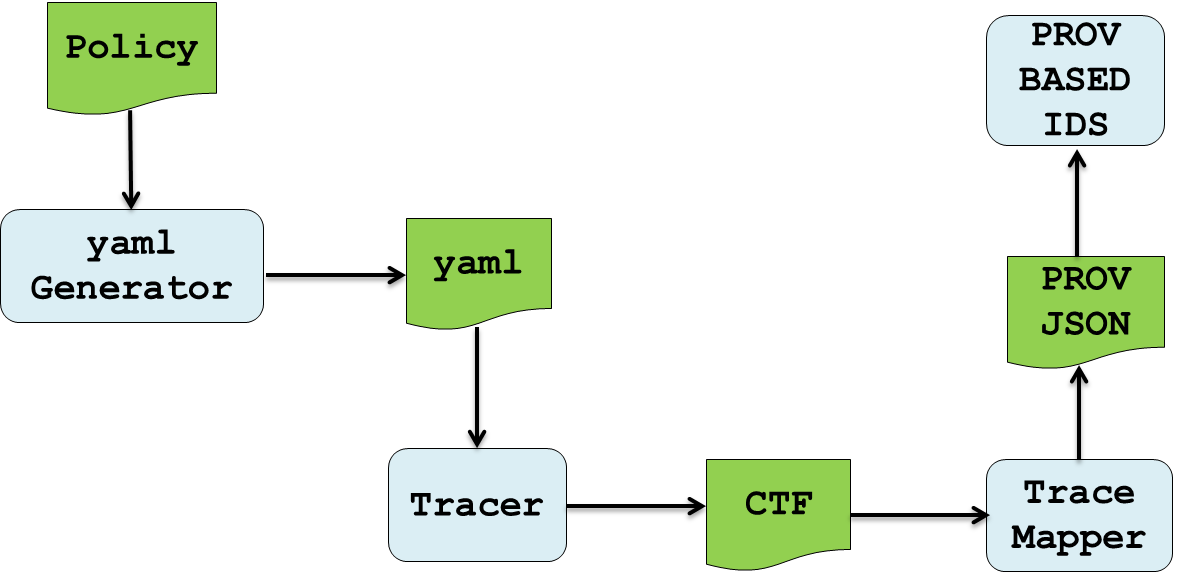
\includegraphics[width =3.0in]{flow.PNG}    
\end{center}
\caption{System Architecture for Provenance Collection.}
\label{architecture}
\end{figure}


\section{Conclusion}
In this paper, we motivate the need for integrating provenance into the IoT architecture. We propose a provenance collection framework that provides provenance collection capabilities for devices in the IoT. 




% conference papers do not normally have an appendix


% use section* for acknowledgment
\section*{Acknowledgment}

The authors would like to thank...





% trigger a \newpage just before the given reference
% number - used to balance the columns on the last page
% adjust value as needed - may need to be readjusted if
% the document is modified later
%\IEEEtriggeratref{8}
% The "triggered" command can be changed if desired:
%\IEEEtriggercmd{\enlargethispage{-5in}}

% references section

% can use a bibliography generated by BibTeX as a .bbl file
% BibTeX documentation can be easily obtained at:
% http://mirror.ctan.org/biblio/bibtex/contrib/doc/
% The IEEEtran BibTeX style support page is at:
% http://www.michaelshell.org/tex/ieeetran/bibtex/
%\bibliographystyle{plain}
% argument is your BibTeX string definitions and bibliography database(s)
%\bibliography{refrences}
%
% <OR> manually copy in the resultant .bbl file
% set second argument of \begin to the number of references
% (used to reserve space for the reference number labels box)

\begin{thebibliography}{1}

\bibitem{IEEEhowto}
H.~Kopka and P.~W. Daly, \emph{A Guide to \LaTeX}, 3rd~ed.\hskip 1em plus
  0.5em minus 0.4em\relax Harlow, England: Addison-Wesley, 1999.

\end{thebibliography}




% that's all folks
\end{document}


